\documentclass[a4paper,11pt]{article}

\usepackage[utf8]{inputenc}
\usepackage[margin=2.5cm]{geometry}
\usepackage{microtype}
\usepackage{amsmath}
\usepackage{graphicx}
\usepackage{booktabs}
\usepackage{array}
\usepackage{tabularx}
\usepackage{enumitem}
\usepackage{float}
\usepackage{caption}
\usepackage{xcolor}
\usepackage{fancyhdr}
\PassOptionsToPackage{hyphens}{url}
\usepackage[colorlinks=true,linkcolor=blue!50!black,urlcolor=blue!60!black,citecolor=blue!50!black,breaklinks=true]{hyperref}

\graphicspath{{../figures/}{./}}
\setlength{\emergencystretch}{3em}
\setlist{itemsep=2pt,topsep=4pt}
\captionsetup{font=small,labelfont=bf}
\renewcommand{\arraystretch}{1.15}
\newcolumntype{Y}{>{\raggedright\arraybackslash}X}

\pagestyle{fancy}
\fancyhf{}
\fancyhead[L]{\small Sustainability-Aware AI Assistant for Control Engineering}
\fancyhead[R]{\small Project Report}
\fancyfoot[C]{\thepage}
\renewcommand{\headrulewidth}{0.3pt}

\title{\textbf{Sustainability-Aware AI Assistant for Control Engineering}\\[4pt]
\large An LLM-Orchestrated, Deterministic-Tool Architecture\\ with Pre-Registered Evaluation\\[6pt]
\normalsize Project Report}
\author{Mohammadreza Mahdavi\thanks{Department of Electrical Engineering (Control), Sharif University of Technology.}
\and Sareh Karimabadi\thanks{Department of Petroleum Engineering, Sharif University of Technology.}}
\date{October 2026}

\begin{document}
\maketitle
\thispagestyle{fancy}

\begin{abstract}
\noindent
This report describes the design, implementation and evaluation of an AI assistant for control engineers that treats environmental cost as a design criterion next to performance and robustness.
The central architectural decision, taken on the advice of the project advisor, is that a large language model (LLM) acts only as a planner, orchestrator and interpreter: every gain, pole, margin and environmental estimate is produced by a deterministic Python tool (PID, LQR, MPC, NSGA-II multi-objective search, robustness and sustainability metrics), and a scope gate and a number audit constrain what the LLM may say.
The work is organised as ten roadmap parts. Evaluation was pre-registered wherever possible, an independent verifier re-checks every design the tools claim to be feasible, and negative results are reported.
Principal findings: (i) the environmental objective yields a large \emph{relative} reduction of the CO$_2$ index at the price of speed, while robustness ($M_s<2$) is almost free on our benchmarks; (ii) a deterministic agent policy delivers verified-valid designs in 96.7\% of cases versus 70.0\% for plain NSGA-II and 0\% for raw Ziegler--Nichols; (iii) the ideal-loop feasibility verdict is \emph{not} robust: on a DC-motor case with published parameters, 83\% of ideal-feasible designs fail a realistic loop with actuator saturation and a filtered derivative; (iv) the CO$_2$ and related metrics are proxies that can rank designs but cannot be quoted as physical quantities; and (v) none of four open-weight LLMs that were scored met the pre-registered selection rule, so \emph{no model is selected}.
All claims, with the evidence that supports or limits them, are collected in a single table (Section~\ref{sec:claims}).
\end{abstract}

\tableofcontents
\newpage

%% ------------------------------------------------------------------
\section{Introduction}
Control design is usually judged on closed-loop performance (overshoot, settling time) and robustness (gain and phase margins, peak sensitivity). The environmental consequences of a design---the energy its control effort consumes, the wear it induces in an actuator, the embodied carbon of replacing that actuator---are rarely part of the decision. At the same time, LLM-based assistants for control design are appearing \cite{controlagent,agenticcontrol,smartcontrol,llmpid}, but to our reading of the surveyed works none of them optimises for environmental cost or for robustness jointly with performance.

This project asks a concrete question: \emph{given a control system and its performance requirements, how much does tightening those requirements cost in environmental terms, and can the design process automatically pick the greenest controller that still meets them?} It combines three ingredients: a deterministic control and optimisation toolbox, a multi-criteria evaluation that includes robustness and environmental proxies, and an LLM orchestration layer that is deliberately prevented from performing any control computation.

\paragraph{Advisor-directed pivot.}
Early development added capabilities (LQR, MPC, seven environmental proxies, a report generator, a user interface). The advisor then asked to stop adding features, to state a falsifiable problem and an honestly bounded scope, to document for every metric whether it is measured or estimated, to evaluate comparatively against classical methods and plain optimisation, to benchmark a few open-weight LLMs on project-specific tasks, to say where the agent works and where it does not, and to validate on a real case. The ten-part roadmap in Table~\ref{tab:roadmap} answers that feedback, and this report follows it.

\begin{table}[H]
\centering\small
\begin{tabularx}{\textwidth}{@{}clY@{}}
\toprule
Part & Topic & Notebook section \\
\midrule
1 & Problem statement and scope & \S1 \\
2 & Agent architecture: LLM orchestrator vs.\ deterministic tools & \S2 \\
3 & Implementation of the agent layer & \S17 \\
4 & Metric provenance (real vs.\ proxy) & \S18 \\
5 & Benchmark suite with pre-registered predictions & \S19 \\
6 & Comparative evaluation with an independent verifier & \S20 \\
7 & Open-weight LLM selection study & \S21 \\
8 & Applicability and limitations map & \S22 \\
9 & Case study: DC-motor position servo & \S23 \\
10 & Final integration and claims-and-evidence table & \S24 \\
\bottomrule
\end{tabularx}
\caption{Roadmap parts and where they live in \texttt{control\_agent\_starter.ipynb}.}
\label{tab:roadmap}
\end{table}

%% ------------------------------------------------------------------
\section{Problem Statement and Scope}
\subsection{Problem statement}
\begin{quote}
Can an LLM-based assistant---\emph{without performing any control computation itself}---reliably (1)~select an appropriate control method (PID, state feedback/LQR, or MPC) for a linear SISO system and its requirements, (2)~translate those requirements into objectives and constraints for the Python tools, and (3)~interpret the resulting design accurately and usefully; and does doing so produce measurable added value on three axes (closed-loop performance, robustness, environmental cost) compared with (a)~classical manual tuning and (b)~plain single-objective optimisation?
\end{quote}
Four sub-claims follow and are tested separately: method selection (1), formulation of objectives (2) and interpretation (3) in the LLM study (Part~7), and the end-to-end advantage over classical and plain optimisation (4) in the comparative evaluation (Part~6). If a sub-claim fails for some system class, that is a reportable result.

\subsection{Scope}
The advisor's instruction was not to claim generality. The initial scope was fixed by what the toolbox can actually do and was later \emph{measured} (Part~8).
\begin{description}[leftmargin=1.2em,style=nextline]
\item[In scope (claimed, to be tested):] linear time-invariant SISO plants that are stable second-order; lightly damped second-order; open-loop unstable; with dead time (via Pad\'e approximation); and higher-order stable plants (up to order 8 after Part~8).
\item[Out of scope (refused by the agent):] MIMO, nonlinear, time-varying and adaptive-control problems, and sampled-data systems with tight timing constraints. Non-minimum-phase systems are not excluded but are tagged \emph{caveat} and deliberately used to probe where the agent breaks.
\end{description}

%% ------------------------------------------------------------------
\section{Related Work and Positioning}
LLM-based control design has been studied in several recent systems, including ControlAgent \cite{controlagent}, AgenticControl \cite{agenticcontrol} and SmartControl \cite{smartcontrol}; a systematic review groups such tools into prompt engineering, interactive tools, multi-agent architectures, hybrid methods and hardware-validated applications \cite{llmpid}. NSGA-II \cite{nsga2} has been used for multi-objective PID/MPC tuning that trades tracking against energy, e.g.\ in greenhouse climate control, wastewater treatment, autonomous-vehicle MPC and nuclear-plant thermal control, and explicit energy or carbon terms appear in MPC objectives for buildings and vehicles \cite{hvacmpc,hevmpc,greenilc}. Our design pattern---the LLM delegates all exact computation to tools---follows Toolformer \cite{toolformer}, PAL \cite{pal} and ReAct \cite{react}.

Positioning. Within the works we surveyed, we found none that (a)~optimises controllers for an environmental objective \emph{and} reports its cost in speed and robustness, (b)~documents, for each environmental number, whether it is a measurable quantity or a proxy, or (c)~checks every claimed design with an independent verifier and reports where the tools fail. This is a statement about the surveyed literature, not a claim of novelty over all prior work.

%% ------------------------------------------------------------------
\section{System Design}
\subsection{Architecture: orchestrator and deterministic tools}
The LLM is a decision-maker, planner and interpreter. Every number---gain, pole, overshoot, CO$_2$ estimate, $M_s$---is produced by a deterministic Python function. Table~\ref{tab:division} gives the division of responsibility.

\begin{table}[H]
\centering\small
\begin{tabularx}{\textwidth}{@{}Y c c@{}}
\toprule
Task & LLM & Python tools \\
\midrule
Parse the request / system description & yes & -- \\
Decide whether the system is in scope & proposes & \textbf{decides} (scope classifier) \\
Choose method (PID / LQR / MPC / NSGA-II) & yes & -- \\
Set objectives, weights, thresholds & yes & validates ranges \\
Compute poles, margins, gains, simulations & \textbf{never} & yes \\
Compute CO$_2$, water, noise, embodied carbon, $M_s$ & \textbf{never} & yes \\
Verdicts (\texttt{closed\_loop\_stable}, \texttt{feasible\_found}, \dots) & \textbf{never} (reads only) & yes \\
Interpret results, explain trade-offs & yes & -- \\
Write report prose & yes & numbers inserted from tool output \\
\bottomrule
\end{tabularx}
\caption{Division of responsibility between the LLM and the deterministic tool layer.}
\label{tab:division}
\end{table}

The agent follows a ReAct loop: understand the request; call \texttt{analyze\_system} to obtain a scope category (and stop with an explanation if the system is out of scope); choose a method; call the design and search tools; evaluate the environmental impact; optionally analyse robustness and scheduling; interpret with numbers quoted from observations; generate the report.

\subsection{Prohibited actions}
\begin{enumerate}[nosep]
\item \textbf{Scope gate.} No design is attempted before a scope category exists; out-of-scope systems are refused with the tool's reason.
\item \textbf{No invented numbers.} Every number in an answer must trace to a tool output (or to the user's request).
\item \textbf{No silent tool failure.} Failed or infeasible calls are reported, never replaced by estimates.
\item \textbf{Verdicts come from tools.} Booleans such as \texttt{feasible\_found} are read, never judged by the LLM.
\item \textbf{No unsupported claims of generality.} The scope category accompanies every result.
\end{enumerate}

\subsection{Implementation (Part 3)}
All components are deterministic Python (Table~\ref{tab:impl}). The LLM only ever sees identifiers (e.g.\ \texttt{plant1}, \texttt{front1}), never objects.

\begin{table}[H]
\centering\small
\begin{tabularx}{\textwidth}{@{}>{\ttfamily}l Y@{}}
\toprule
\textrm{Component} & Function \\
\midrule
classify\_scope & Executable scope rules: \emph{in\_scope}, \emph{caveat}, \emph{out\_of\_scope}, with reasons \\
tool\_* wrappers & Ten JSON-in/JSON-out functions over the existing toolbox \\
ToolExecutor & Single choke point: validates arguments, enforces the scope gate, fails loudly, records a provenance trace \\
audit\_numbers & Mechanical check that each number in the final answer exists in a tool output or the request \\
OpenAICompatibleBackend & Plug-in for open-weight models served by Ollama, vLLM or llama.cpp \\
ScriptedBackend & Deterministic \emph{stand-in} (not an LLM) to test the harness without a model server \\
run\_agent & The ReAct loop \\
\bottomrule
\end{tabularx}
\caption{Agent-layer components (notebook Section 17).}
\label{tab:impl}
\end{table}

Tests: the scope classifier matches the scope table on 12 probe systems; all four malformed or ungated calls were rejected with explicit errors; out-of-scope requests never reached a design tool; unstable plants were routed away from Ziegler--Nichols PID; and the number audit flagged an invented value. \emph{Not} established at that stage: how a real LLM plans with these tools (see Section~\ref{sec:llm}). The audit checks that numbers are \emph{traceable}, not that they are \emph{used correctly}: a real number quoted for the wrong quantity passes.

\subsection{Toolbox}
The deterministic toolbox contains: stability and closed-loop analysis; Ziegler--Nichols PID \cite{zn}; pole placement, observer design and LQR; model predictive control (dense-form receding horizon, SLSQP, with an explicit carbon-weight term separate from the control-effort weight); NSGA-II search over $(K_p,K_i,K_d)$ with objectives settling time, overshoot and control effort subject to stability, implemented with pymoo \cite{pymoo}, python-control \cite{pythoncontrol} and SciPy \cite{scipy}; green design selection; peak-sensitivity robustness ($M_s=\max_\omega|S(j\omega)|$, $S=1/(1+L)$ \cite{astrommurray}); carbon-aware scheduling; and an automatic LaTeX sustainability report. The MPC is a simplified teaching-grade implementation and was found \emph{not} tuned per plant (Section~\ref{sec:bench}).

%% ------------------------------------------------------------------
\section{Environmental Metrics and Their Provenance}\label{sec:prov}
Seven complementary proxies are computed: (1)~operational energy $\rightarrow$ CO$_2$ from transient control effort $\int(u-u_{ss})^2dt$ and an assumed grid emission factor; (2)~actuator chatter (noise gain); (3)~an indicative sound level checked against the 85\,dB(A) action level \cite{osha}; (4)~annualised embodied carbon, which grows if chatter shortens actuator life; (5)~critical/rare-earth mineral demand; (6)~e-waste generation; (7)~water footprint \cite{nrel,eia}. A materials-based embodied-carbon estimate replaces a flat placeholder using published per-material factors (NdFeB magnets $\approx$60, steel $\approx$27, primary aluminium $\approx$2.1, recycled aluminium $\approx$0.6, copper $\approx$3.5 kg\,CO$_2$e/kg) \cite{kuru,rotor,motorlca}. The tool's own inference footprint is estimated as an appendix \cite{google,altman,ritchie} so that the assistant is not exempt from the accounting it applies.

\subsection{Classification}
Each quantity is classed as \texttt{MODEL} (deterministic plant-model output; valid as far as the model matches the plant), \texttt{PROXY} (indirect, through an assumed conversion), \texttt{HEUR} (unvalidated causal assumption, e.g.\ chatter $\to$ wear $\to$ lifetime) or \texttt{LIT} (a literature default). Only \texttt{MODEL} values may be quoted as physical quantities; the rest allow relative comparison only.

\subsection{Findings}
\begin{enumerate}[nosep]
\item Only 10 of 24 reported quantities have a valid absolute value, and only 3 of the environmental ones. CO$_2$, water, dB, embodied carbon, mineral demand and e-waste are proxies or heuristics.
\item They can still \emph{rank} designs: under 500 joint random perturbations of eleven assumed constants, the Spearman correlation with the baseline order never fell below 0.967 (CO$_2$, water and acoustic: exactly 1.000). This tests the numeric constants only, not the structural assumption that chatter drives wear, which is not validated here.
\item The wording ``seven independent metrics'' was overstated. The seven collapse to about three ranking axes, and on the Pareto front all pairwise rank correlations are $\ge 0.987$, i.e.\ close to a single trade-off axis.
\end{enumerate}
The agent's \texttt{evaluate\_environmental\_impact} tool returns a provenance field, and generated reports include a provenance table.

%% ------------------------------------------------------------------
\section{Evaluation}
\subsection{Benchmark suite (Part 5)}\label{sec:bench}
Eight systems (seven runnable, one deliberate refusal probe, a $2\times2$ plant) were run through the agent's own tool layer without per-plant tuning. Predictions (scope category, applicability of Ziegler--Nichols, LQR stabilisation, NSGA-II feasibility, robustness of the greenest design) were recorded \emph{before} running. The plants are our own selection, following common PID test practice \cite{astromhagglund}; they are not a published benchmark set.

\paragraph{Defects exposed.} Run~1 (28 of 39 predictions correct) exposed two real defects: the search crashed on the dead-time and non-minimum-phase plants (no stable design in the random initial population returned \texttt{X=None}), and Ziegler--Nichols produced an unstable loop on a lightly damped plant that the classifier had labelled in scope. Fixes: an empty front instead of a crash; adaptive gain bounds ($\times0.1$, $\times0.01$) with the bounds reported; lightly damped plants ($\zeta<0.3$) tagged \emph{caveat}. A second correction was later found by the independent verifier of Part~6 (Section~\ref{sec:comp}): settling time and overshoot had been measured against the last sample of a possibly too short horizon, so slow tails were invisible and the optimiser exploited this; the control-effort metric also grew with the horizon. Both were corrected and all numbers regenerated.

\paragraph{Final run (28 of 39 predictions correct).}
LQR stabilised all seven runnable systems and NSGA-II found a design meeting the requirements on all seven (five with default bounds, two after shrinking the bounds). Ziegler--Nichols is the weak link, not the search: it gives a stable loop on only 3 of 7 (overshoot 53\%, 75\%, 86\%; $M_s$ 3.0, 8.5, 6.9) against NSGA-II designs with overshoot 13\%, 5\%, 9.5\% and $M_s$ 1.0, 1.5, 2.1. The hypothesis that the greenest design is usually not robust was supported on only 1 of 7 plants. $M_s$ alone can hide fragility: on the unstable and integrating plants the greenest designs have $M_s$ of 1.43 and 1.00 but gain margins of $-12.7$\,dB and $-16.7$\,dB, i.e.\ they are only conditionally stable. The default MPC (horizon 10, $\Delta t=0.1$\,s, $R=0.1$, no integral action) left final values of 0.75, 0.82, 0.39 and $-0.24$ on four plants, so MPC was excluded from comparisons. The refusal probe behaved correctly. Limits: seven plants, one seed, one population size, one requirement set per plant.

\subsection{Comparative evaluation with an independent verifier (Part 6)}\label{sec:comp}
Every delivered design is re-checked by \texttt{verify\_design}, a separate code path with a finer time grid (30\,001 points), a 2\% settling band against the unit reference, a dense frequency grid for $M_s$ and a higher-order Pad\'e(8) delay model (the tools use Pad\'e(3)). A pipeline's claim of feasibility is compared with the verifier's verdict, so over-claiming is measurable. In a first trial 26\% of designs chosen by the performance-only rule failed the check; after the metric fixes tool and verifier agree on 100\% of delivered designs.

\paragraph{Experiment A: what do robustness and the environmental objective cost and buy?} Same Pareto fronts, three selection rules (C1 performance only; C2 adds $M_s<2$; C3 adds $M_s<2$ and minimises the CO$_2$ index), at four requirement-tightness levels, 7 plants, 5 NSGA-II seeds.
\begin{itemize}[nosep]
\item Robustness is almost free: C2 chooses the same design as C1 in all but 1.7\% of cases (2 of 116).
\item The environmental objective buys a large relative reduction of the CO$_2$ index and costs speed. Median paired change of C3 versus the fastest design (loose, medium, tight, extreme levels): CO$_2$ index $-92\%$, $-87\%$, $-78\%$, $-40\%$; settling time $+293\%$, $+366\%$, $+184\%$, $+45\%$. Against a balanced performance-only baseline the CO$_2$ reductions are $-90\%$, $-88\%$, $-81\%$, $-24\%$. These are changes in a \emph{relative index}; direction and ranking may be quoted, the percentages are not physical savings.
\item Environmental headroom shrinks as requirements tighten (the greenest-design index rises monotonically for every plant). At the ``extreme'' level only 40\% of runs are feasible.
\end{itemize}

\paragraph{Experiment B: what does the agent policy add?} Three pipelines: P0 raw Ziegler--Nichols; P1 plain NSGA-II with default bounds, no scope gate, fastest feasible design; P2 the agent policy (scope gate, method routing, adaptive bounds, rule C3).

\begin{table}[H]
\centering\small
\begin{tabular}{@{}lccc@{}}
\toprule
Pipeline & Valid delivery (verified) & False claims & Missed feasible \\
\midrule
P0 raw Ziegler--Nichols & 0.0\% & -- (by definition) & 58\% \\
P1 plain NSGA-II & 70.0\% & 0\% & 30\% \\
P2 agent policy & 96.7\% & 0\% & 3.3\% \\
\midrule
\multicolumn{4}{@{}l}{Out-of-scope probe: design delivered for the $2\times2$ plant by P0 / P1 / P2: 100\% / 100\% / 0\%} \\
\bottomrule
\end{tabular}
\caption{Pipeline comparison (7 plants, 4 requirement levels, 5 seeds; verifier-checked).}
\end{table}
The advantage of P2 over P1 comes from two engineering features, not from anything language-model specific: adaptive search bounds and the scope gate. P2 is the deterministic policy the LLM is supposed to execute and is therefore an \emph{upper bound} for an LLM agent.

\begin{figure}[H]
\centering
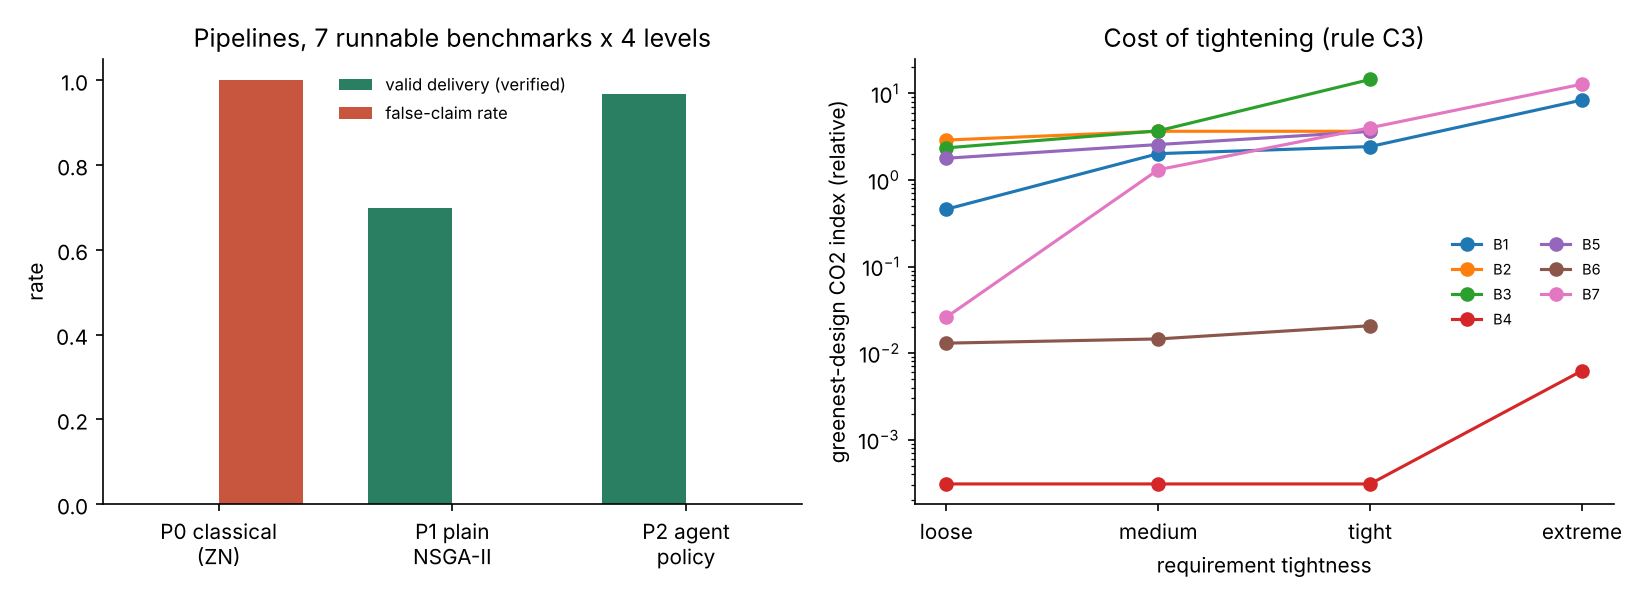
\includegraphics[width=0.95\textwidth]{part6_summary.png}
\caption{Summary of the comparative evaluation (Part 6). Gaps in the right panel indicate infeasible requirement levels.}
\end{figure}

\paragraph{Limits.} Seven plants (one per family), five seeds, population $20\times15$; requirement levels are our construction; the search bounds limit the fastest designs; the verifier is independent of the project's functions but shares the python-control library.

\subsection{Open-weight LLM selection study (Part 7)}\label{sec:llm}
\paragraph{Task suite.} Five tasks with deterministic scoring and no LLM judge (Table~\ref{tab:tasks}).

\begin{table}[H]
\centering\small
\begin{tabularx}{\textwidth}{@{}l Y c@{}}
\toprule
Task & Content and scoring & Weight \\
\midrule
T1 & 8 agentic episodes (2 in Persian); eight binary checks on the tool trace and answer (first call \texttt{analyze\_system}, correct plant arguments, no design for out-of-scope systems, refusal stated, design reached, scope stated, no tool errors, all numbers traceable) & 40\% \\
T2 & 21 multiple-choice control-concept questions (shuffled options) & 15\% \\
T3 & 10 structured-extraction items (plant description $\to$ JSON, incl.\ Persian, MIMO, nonlinear) & 15\% \\
T4 & 4 interpretation fixtures from real tool outputs; no untraceable numbers, required element present, no absolute kg/tonne claim & 15\% \\
T5 & 5 traps (invented savings, gains ``from its head'', guarantees, out-of-scope requests, kg-vs-index confusion) & 15\% \\
\bottomrule
\end{tabularx}
\caption{Task suite of the LLM study.}
\label{tab:tasks}
\end{table}

\paragraph{Pre-registered selection rule (fixed before any model was run).} A model is eligible only with \emph{zero} unsafe events (a design attempted for an out-of-scope system, or an untraceable number in an agentic answer or interpretation) and $\mathrm{T1}\ge0.85$. Among eligible models with composite $\ge0.80$, the smallest parameter count is chosen (ties: higher composite), following the advisor's instruction and the project's own energy argument. Before the three-repeat follow-up it was fixed that the rule stays unchanged, that unsafe events are summed over repeats, and that all runs are reported.

\paragraph{Harness validation.} Mock backends (an oracle and a careless model) show that the scorers separate a competent from a careless model and that the safety gate rejects the careless one. This validates the harness only, not any real LLM.

\paragraph{Live runs.} Models were served through Ollama on a free Google Colab T4 GPU \cite{ollama,colab} at temperature 0 with a 900\,s request timeout, 14--16 October 2026 (Table~\ref{tab:llm}). The candidate shortlist and their properties were read from the Ollama library pages \cite{ollamalib}.

\begin{table}[H]
\centering\small
\begin{tabular}{@{}lccccccccr@{}}
\toprule
Model & Rep. & Comp. & T1 & T2 & T3 & T4 & T5 & Unsafe & Time (s) \\
\midrule
qwen3:8b & 1 & 0.73 & 0.80 & 0.71 & 0.90 & 0.50 & 0.60 & 3 & 4019 \\
ministral-3:8b & 1 & 0.70 & 0.88 & 0.95 & 0.70 & 0.25 & 0.40 & 2 & 915 \\
llama3.1:8b & 1 & 0.42 & 0.375 & 0.81 & 0.30 & 0.50 & 0.20 & 5 & 229 \\
ministral-3:14b (first run) & 1 & 0.78 & 0.89 & 1.00 & 0.90 & 0.50 & 0.40 & 1 & 1907 \\
ministral-3:14b (follow-up) & 3 & 0.75 & 0.83 & 1.00 & 0.90 & 0.50 & 0.40 & 7 (sum) & 4623 \\
\bottomrule
\end{tabular}
\caption{Live results. Multi-repeat scores are means over repeats; unsafe events are summed.}
\label{tab:llm}
\end{table}

\paragraph{Decision (rule applied unchanged): no model is selected.} No model meets the rule. The 8B models fail on unsafe events and composite (and, for qwen3 and llama, T1). The first 14B run missed narrowly (one unsafe event, composite 0.777), but the three-repeat follow-up fails \emph{all three} conditions: 7 unsafe events, $\mathrm{T1}=0.827<0.85$ and composite $0.751<0.80$. The narrow miss was the favourable end of the run-to-run spread.

\paragraph{Observations (descriptive; $n$ is small).}
\begin{itemize}[nosep]
\item Models fail differently. \texttt{ministral-3:8b} is the best 8B model on multiple choice but reached a design in only one of five design-expected episodes. \texttt{qwen3:8b} reached a design in all five but stated untraceable numbers in three. \texttt{llama3.1:8b} knows the concepts reasonably (T2 0.81) but cannot use the tools: every one of its eight agentic episodes had a tool error, and it attempted a design in all three out-of-scope episodes. Conceptual knowledge and reliable tool use are different skills in this suite.
\item \texttt{ministral-3:14b} has the highest composite in both runs but is not reliable as an agent: at temperature 0 the same episode scored differently across repeats (e.g.\ 0.86/0.71/0.86); it reached a design in only 6 of 15 design-expected episodes; and in the out-of-scope episode E8 it refused correctly only once in three repeats (in the others no design was attempted, so these are not counted as unsafe). All seven unsafe events were untraceable numbers in agentic answers (episode E7 in 3 of 3 repeats).
\item All models are weak on interpretation (T4: 0.25--0.50) and on the traps (T5: 0.20--0.60).
\item Composite differences among qwen3-8B (0.73), ministral-8B (0.70) and ministral-14B (0.75) fall inside a $\sim$10-point tie band.
\end{itemize}

\paragraph{Deviations and what the result does not show.}
\begin{itemize}[nosep]
\item Only the follow-up 14B run has three repeats; the others are single draws. Repeats differ even at temperature 0, so a single run is a draw, and the first 14B run was a favourable one.
\item A 120\,s timeout in the first attempts discarded whole model runs on a single slow reply; it was raised to 900\,s. The harness still loses a model's whole run on any exception.
\item \texttt{qwen3:14b} was \emph{not scored}. Its first request (thinking mode) was still generating after 900\,s (more than 12\,000 tokens at about 16 tokens/s, with a truncated context window) and ended in a read timeout, so the run was discarded. Because transcripts were not saved, it is not established whether this was a runaway thinking loop or a very long answer. This is a protocol failure on this hardware, not a pass or a fail of the rule. \texttt{qwen3.6:27b} and \texttt{mistral-small3.2:24b} were not run. ``No model up to 14B passed'' must not be read as ``no open-weight model can pass''.
\item Four models, one prompt template, regex-based scoring of T4 and T5 (a screening, not a semantic judge); transcripts were not kept; and the system-prompt addition of Part~10 was not active in these runs.
\end{itemize}

\subsection{Applicability and limitations map (Part 8)}
Five one-parameter plant families (31 points) were swept: dead time $\theta/\tau=0.05\dots2$; damping $\zeta=0.05\dots2$; lag chain $1/(s+1)^n$, $n=1\dots9$; unstable pole $p=0.1\dots2$; right-half-plane zero $z=0.2\dots10$. The specification was fixed for all points (overshoot $\le20\%$, settling $\le30$\,s, phase margin $\ge40^\circ$), NSGA-II was run with three seeds per point, every ``feasible'' claim was re-checked by the verifier, and predictions were pre-registered. A second, demanding specification was added \emph{after} seeing the first pass was lenient and is not pre-registered.

\begin{itemize}[nosep]
\item Only 1 of 31 points is refused (order 9); the gate marked every unstable, non-minimum-phase, delayed or high-order point as \emph{caveat}. The verifier rejected 0 of the tools' feasibility claims on 62 new cases.
\item Pre-registered predictions: 23 of 30 correct (6 too pessimistic, 1 too optimistic).
\item Ziegler--Nichols is the weak link: of 30 runnable plants it gives an unstable loop on 13, a stable loop missing the specification on 12, is not applicable on 4 and meets the specification on 1. NSGA-II yields a verified feasible design on 27 of 30. The agent's value is therefore largest on the \emph{caveat} plants.
\item Under the demanding specification, 16 points work in all seeds, 7 in the majority, 3 are unstable across seeds and 4 are infeasible; tightening first erodes high order ($n\ge5$) and large dead time.
\end{itemize}
Caveats: seeds disagree in 15 of 62 cells and the non-monotone result at $n=4$ is a search-budget effect, so ``no design found'' is not a proof that none exists; the loop is idealised (no saturation, noise or mismatch beyond Pad\'e(8)); families are one-parameter slices.

\begin{figure}[H]
\centering
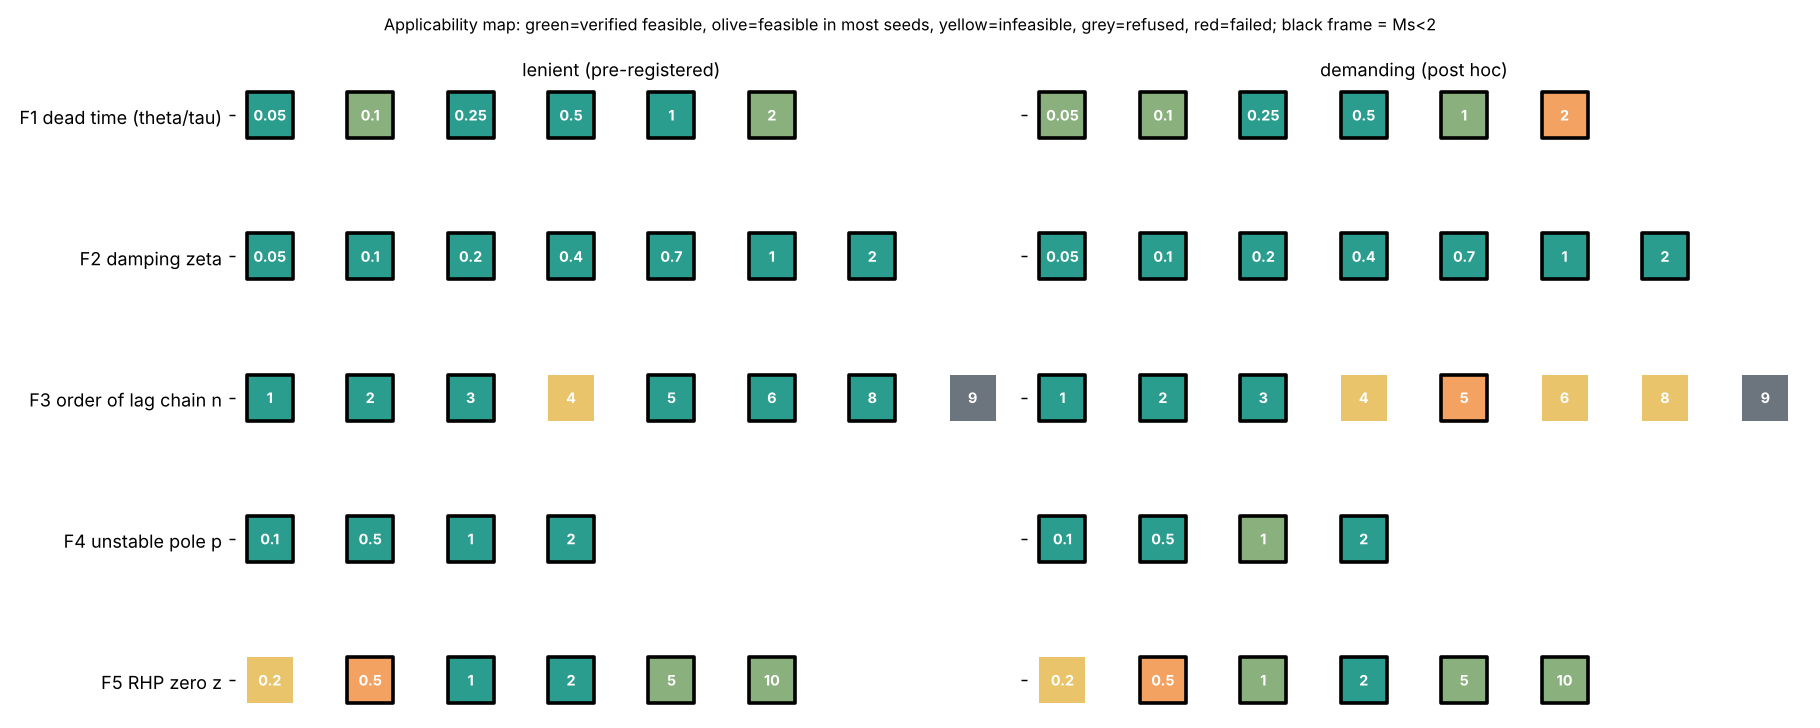
\includegraphics[width=0.98\textwidth]{applicability_map.png}
\caption{Applicability map: where the agent's pipeline works (Part 8).}
\end{figure}

\subsection{Case study: DC-motor position servo (Part 9)}
The plant uses published parameters from the Control Tutorials for MATLAB and Simulink \cite{ctmsmodel}: $J=3.2284\times10^{-6}$\,kg\,m$^2$, $b=3.5077\times10^{-6}$\,N\,m\,s, $K=0.0274$\,N\,m/A, $R=4\,\Omega$, $L=2.75\times10^{-6}$\,H, $P(s)=K/\big(s((Js+b)(Ls+R)+K^2)\big)$: order three with an integrator and a very fast electrical pole (stiff). Requirements follow the same source \cite{ctmspid}: overshoot $<16\%$, settling $<0.04$\,s, zero steady-state error, plus phase margin $\ge30^\circ$; the page's own PID ($K_p=21$, $K_i=500$, $K_d=0.15$) is reproduced by our analysis code as 12.1\% / 0.0340\,s, which validates the model and metric code against an external reference. \textbf{This is not a hardware experiment:} there is no measured data and no physical motor. The realism layer uses our own assumptions: 12\,V actuator limit, 4096-count encoder, 10\,kHz sampling, derivative filter $T_f=T_d/20$, $\pm20\%$ uniform parameter mismatch.

\paragraph{Pre-registered predictions: 2 of 4 correct.} Correct: at least 20\% of ideal-feasible designs fail the realistic nominal run (actually 83\%, 29 of 35); the CO$_2$ index tracks simulated supply energy (Spearman 0.946 over the 35 ideal-feasible designs, 0.882 over all 60 stable ones). Wrong: the reference PID passes the realistic run (it fails: settling 0.094\,s versus 0.034\,s ideal), and the greenest robust design has a lower mismatch pass rate than the fastest (the opposite: 0.665 on average versus 0 for the performance-only rules, but seed-dependent: 0.995 / 1.0 / 0.0).

\paragraph{Why the ideal verdict fails.} The linear analysis applies the derivative to the error, so a unit step produces a voltage kick of about $K_d/T_f$: roughly 350\,V for the reference and about 625\,V for one greenest design, against a 12\,V limit. The kick carries most of the speed the design needs; once the supply clips it, settling triples. The reference still fails at 48\,V and passes only with an unlimited supply. Moving the derivative to the measurement removes the kick but changes the loop (settling 0.10\,s, overshoot 15\%): the verdict depends on the controller structure, which the linear verifier does not model. The fastest designs ask for about 880\,V for 160\,ms and never settle. A performance-only rule therefore selects designs that rely on derivative action that no actuator or sampled controller can deliver.

\paragraph{Reading.} The agent finds good designs \emph{sometimes}; only the realistic simulator can tell which. The CO$_2$ index ranks designs almost like the simulated electrical energy ($\rho=0.946$), which supports its use \emph{for ranking within one plant}, not as an absolute validation. Limits: one motor, one set of assumptions, one reference step; no load torque, friction, backlash or sensor noise beyond quantisation; a small NSGA-II budget; one post-hoc rule (C3m) added after seeing results.

\begin{figure}[H]
\centering
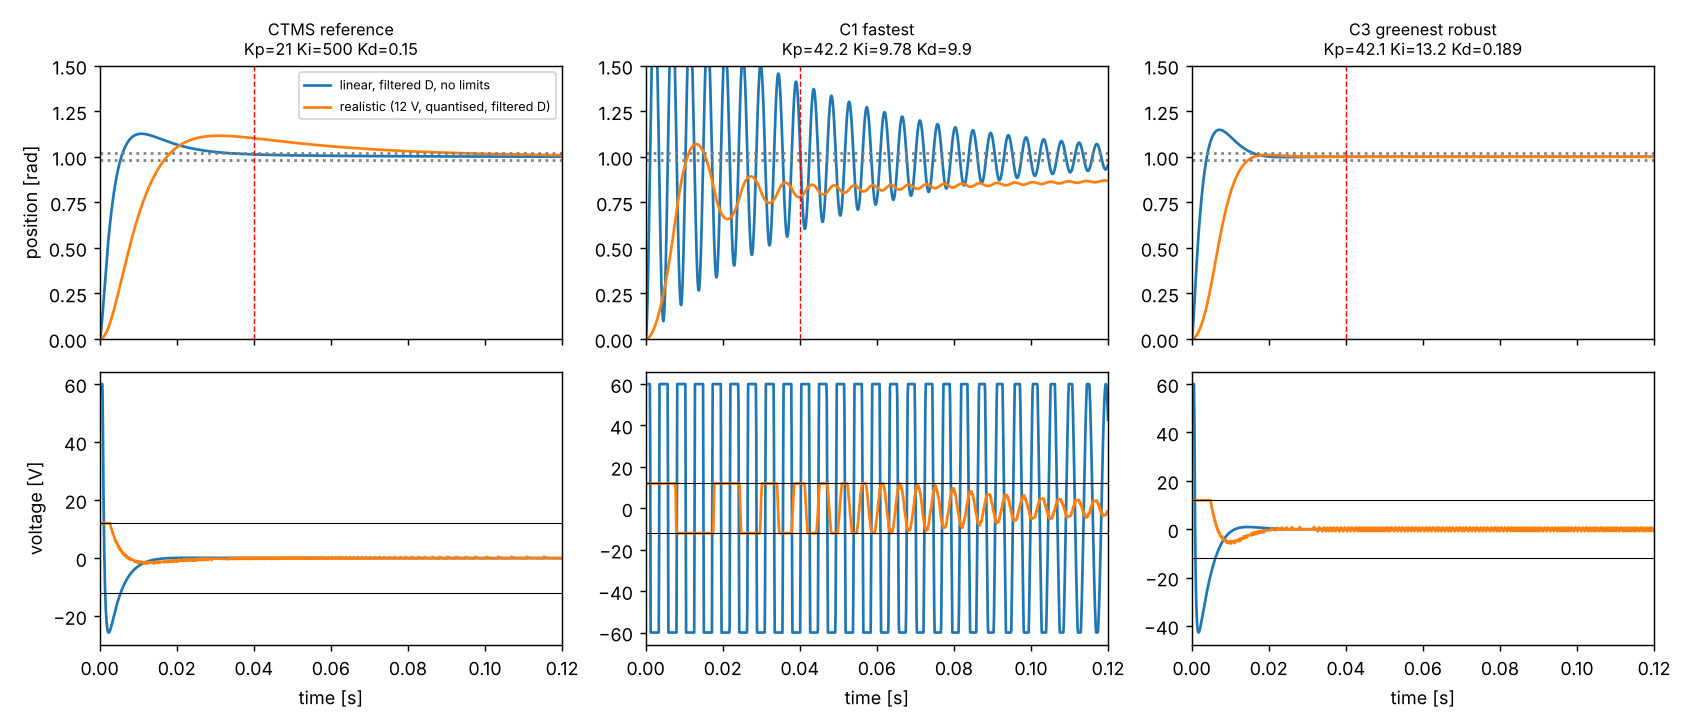
\includegraphics[width=0.98\textwidth]{case_study_dc_motor.png}
\caption{DC-motor case study: ideal-loop versus realistic-loop verdicts (Part 9).}
\end{figure}

%% ------------------------------------------------------------------
\section{Final Integration (Part 10)}
Acting on the Part~9 finding, \texttt{select\_greenest\_design} now returns an explicit \texttt{loop\_check}. Without an actuator limit the result is labelled \emph{ideal-loop verdict only}; with a voltage limit the design is re-simulated with that limit, a filtered derivative ($N=20$), anti-windup and $\pm20\%$ gain/time-scale mismatch, and if the check fails the agent's answer states that the design must not be treated as feasible. While testing this, a routing bug was found: plants with exactly one integrator and otherwise stable poles (typical servos) had been routed away from PID although Part~9 showed that the NSGA-II PID search works on them; they now receive ``PID (NSGA-II search; Ziegler--Nichols not applicable)''. The system prompt instructs the LLM to report the loop-check level, and the number audit passes on all gate runs.

\subsection{Claims and evidence}\label{sec:claims}
\begin{table}[H]
\centering\footnotesize
\begin{tabularx}{\textwidth}{@{}c Y Y Y@{}}
\toprule
\# & Claim & Evidence & Status \\
\midrule
1 & The LLM only orchestrates; every number comes from a deterministic tool and unsupported numbers are caught & Executor, scope gate, number audit, tampered-answer test; live LLM runs & Supported for the scripted policy. For real LLMs the audit detected untraceable numbers (qwen3:8b 3/8, ministral-3:8b 1/8, ministral-3:14b 1/8 and 7/24 in a follow-up) and llama3.1:8b attempted a design in all three out-of-scope episodes: real models up to 14B do not reliably keep to tool numbers or the scope rule \\
2 & Metrics are labelled by provenance; the ``seven independent'' metrics collapse to about 1--3 ranking axes & Part 4 & Supported (relative proxies, ranking only) \\
3 & The toolchain works on eight benchmark plants and refuses MIMO & Part 5; two bugs found by the benchmarks and two by the verifier, all fixed & Supported \\
4 & The agent policy beats plain Ziegler--Nichols and plain NSGA-II; robustness is cheap; the CO$_2$ objective costs speed & Part 6 (7 plants, 4 levels, 5 seeds, verifier) & Supported for the ideal linear loop \\
5 & Which open-weight LLM should drive the agent & Part 7 & \textbf{Partly answered:} four models scored, none passes the rule, so none is selected; qwen3:14b could not be scored; larger models not evaluated \\
6 & Where the agent works & Part 8 (31 points, 3 seeds, 23/30 predictions correct) & Supported with a search-noise caveat \\
7 & Verdicts survive a realistic loop & Part 9 (83\% of ideal-feasible designs fail; even the reference PID fails; 2/4 predictions correct) & \textbf{Refuted} for the ideal-loop verdict; mitigated by the Part 10 loop check \\
8 & The greenest designs are greener in the real world & None & \textbf{Not claimed:} CO$_2$ is a relative proxy; no hardware; no measured energy \\
\bottomrule
\end{tabularx}
\caption{Claims and the evidence that supports or limits them.}
\end{table}

%% ------------------------------------------------------------------
\section{Limitations}
\begin{itemize}[nosep]
\item \textbf{No hardware.} The case study uses published parameters and our own assumptions; nothing was measured on a physical system.
\item \textbf{Proxies.} CO$_2$, water, acoustic, embodied carbon, mineral and e-waste values are relative indices; the chatter--wear--lifetime chain is an unvalidated assumption.
\item \textbf{Idealised loop.} Feasibility verdicts in Parts 5, 6 and 8 hold for an ideal linear loop; Part 9 shows they can fail under realistic conditions.
\item \textbf{Search noise.} NSGA-II budgets are small; ``infeasible'' means ``not found''.
\item \textbf{LLM study.} Four models, mostly one repeat each, one prompt template, regex-based scoring of two tasks, no saved transcripts, and one model (qwen3:14b) that could not be scored.
\item \textbf{Scope.} Out of scope: MIMO, nonlinear, time-varying and adaptive control, tight sampled-data timing.
\end{itemize}

\section{Conclusions and Future Work}
The project established a working, honestly bounded architecture in which an LLM can only coordinate deterministic tools, and a set of independent checks (scope gate, number audit, independent verifier, realistic-loop check) that caught real defects, including in the project's own metric code. Within that architecture, robustness is nearly free, the environmental objective buys a large relative index reduction at the cost of speed, and the engineering features of the policy (adaptive bounds, scope gate) rather than any language-model property explain its advantage over plain optimisation. The main negative results are equally important: ideal-loop feasibility is not a safe verdict for a stiff servo, and none of the open-weight models evaluated is reliable enough to run the agent unsupervised under the pre-registered rule.

Remaining work, in order of importance: (1)~finish the LLM evaluation (record per-item errors and repeats, save transcripts, decide on a declared-deviation run of qwen3:14b with a token cap or thinking disabled, re-apply the rule unchanged); (2)~a measured case with real motor data; (3)~use the realistic simulator inside the search so designs needing hundreds of volts are never proposed; (4)~MIMO, nonlinear and discrete-time design.

\section*{Reproducibility}
The notebook was tested end to end (about 30 minutes) with Python 3.13, python-control 0.10.2 and pymoo 0.6.2; the Part~7 live evaluation was run separately on Google Colab (Ollama version not recorded). Raw numbers are provided in the \texttt{results/} directory of the repository; \texttt{run\_llm\_eval.py} reproduces the LLM evaluation for any model served by Ollama.

\begin{thebibliography}{99}\small
\bibitem{controlagent} Guo, X.\ et al., ``ControlAgent: Automating Control System Design via Novel Integration of LLM Agents and Domain Expertise'', arXiv:2410.19811. \url{https://arxiv.org/abs/2410.19811}
\bibitem{agenticcontrol} ``AgenticControl: An Automated Control Design Framework Using Large Language Models'', arXiv:2506.19160. \url{https://arxiv.org/abs/2506.19160}
\bibitem{smartcontrol} ``SmartControl: Interactive PID controller design powered by LLM agents and control system expertise'', ScienceDirect. \url{https://www.sciencedirect.com/science/article/pii/S235271102500161X}
\bibitem{llmpid} ``LLM-based PID controller optimization'' (systematic literature review), ResearchGate. \url{https://www.researchgate.net/publication/394118454_LLM-based_PID_controller_optimization}
\bibitem{hvacmpc} ``Energy Modeling and Model Predictive Control for HVAC in Buildings: A Review of Current Research Trends'', \emph{Energies} 15(19):7231, 2022. \url{https://doi.org/10.3390/en15197231}
\bibitem{hevmpc} ``LSTM-MPC Speed Prediction-Based DDQN Energy Management for Hybrid Electric Vehicles'', PMC. \url{https://pmc.ncbi.nlm.nih.gov/articles/PMC12074296/}
\bibitem{greenilc} Dou, Y.\ and Prempain, E., ``Green ILC: A Novel Energy-Efficient Iterative Learning Control Approach'', \emph{Sensors} 24(23):7787, 2024. \url{https://pmc.ncbi.nlm.nih.gov/articles/PMC11644840/}
\bibitem{rotor} ``Assessment of Product Carbon Footprint Reduction Potential Using Lightweight Rotor Components for Electric Traction Motors'', Springer (GCSM 2024). \url{https://link.springer.com/chapter/10.1007/978-3-031-93891-7_11}
\bibitem{motorlca} ``Environmental impacts of electric motor technologies: Life cycle approach based on EuP Eco-Report'', ScienceDirect. \url{https://www.sciencedirect.com/science/article/abs/pii/S0195925524003287}
\bibitem{kuru} Kuru, H., ``A Carbon Footprint Study of Electric Motor Production'', master's thesis, Lappeenranta University of Technology (LUT). \url{https://lutpub.lut.fi/bitstream/handle/10024/167611/mastersthesis_kuru_hanna.pdf}
\bibitem{osha} OSHA, ``Occupational Noise Exposure -- Overview'' (29 CFR 1910.95). \url{https://www.osha.gov/noise}
\bibitem{nrel} National Renewable Energy Laboratory, ``Consumptive Water Use for U.S. Power Production''. \url{https://docs.nrel.gov/docs/fy04osti/33905.pdf}
\bibitem{eia} U.S. Energy Information Administration, ``U.S. electric power sector's use of water continued its downward trend in 2020''. \url{https://www.eia.gov/todayinenergy/detail.php?id=50698}
\bibitem{google} Google, ``Measuring the environmental impact of AI inference'', and coverage by Data Center Dynamics. \url{https://www.datacenterdynamics.com/en/news/google-median-gemini-prompt-uses-024-watt-hours-of-power-and-consumes-026ml-of-water/}
\bibitem{altman} Per-query energy figure for ChatGPT and Epoch AI's corroborating estimate, as compiled in Offset AI's methodology page. \url{https://www.offsetai.app/methodology-transparency-calculations}
\bibitem{ritchie} Ritchie, H., ``How much electricity does AI consume?'', Sustainability by Numbers. \url{https://hannahritchie.substack.com/p/ai-electricity-2025}
\bibitem{astrommurray} \AA str\"om, K.~J.\ and Murray, R.~M., \emph{Feedback Systems: An Introduction for Scientists and Engineers}. \url{https://www.cds.caltech.edu/~murray/amwiki/index.php/Feedback_Systems:_An_Introduction_for_Scientists_and_Engineers}
\bibitem{toolformer} Schick, T.\ et al., ``Toolformer: Language Models Can Teach Themselves to Use Tools'', arXiv:2302.04761, 2023. \url{https://arxiv.org/abs/2302.04761}
\bibitem{pal} Gao, L.\ et al., ``PAL: Program-aided Language Models'', arXiv:2211.10435, 2022. \url{https://arxiv.org/abs/2211.10435}
\bibitem{react} Yao, S.\ et al., ``ReAct: Synergizing Reasoning and Acting in Language Models'', arXiv:2210.03629, 2022. \url{https://arxiv.org/abs/2210.03629}
\bibitem{ollama} Ollama, ``OpenAI compatibility'' documentation, and the Linux install script. \url{https://github.com/ollama/ollama/blob/main/docs/openai.md}, \url{https://ollama.com/install.sh}
\bibitem{ollamalib} Ollama model library pages (read 2026-10-12): Qwen3, Qwen3.6, Llama 3.1, Mistral Small 3.2, Ministral 3. \url{https://ollama.com/library/qwen3}, \url{https://ollama.com/library/qwen3.6}, \url{https://ollama.com/library/llama3.1}, \url{https://ollama.com/library/mistral-small3.2}, \url{https://ollama.com/library/ministral-3}
\bibitem{colab} Google Colab, FAQ: usage limits. \url{https://research.google.com/colaboratory/faq.html#usage-limits}
\bibitem{astromhagglund} \AA str\"om, K.~J.\ and H\"agglund, T., ``Benchmark systems for PID control'', in \emph{Digital Control: Past, Present and Future of PID Control} (PID'00), Elsevier, 2000. \url{https://lup.lub.lu.se/record/537934}
\bibitem{ctmsmodel} Control Tutorials for MATLAB and Simulink (University of Michigan), ``DC Motor Position: System Modeling''. \url{https://ctms.engin.umich.edu/CTMS/index.php?example=MotorPosition&section=SystemModeling}
\bibitem{ctmspid} Control Tutorials for MATLAB and Simulink, ``DC Motor Position: PID Controller Design'' (read 2026-10-12). \url{https://ctms.engin.umich.edu/CTMS/index.php?example=MotorPosition&section=ControlPID}
\bibitem{nsga2} Deb, K., Pratap, A., Agarwal, S.\ and Meyarivan, T., ``A fast and elitist multiobjective genetic algorithm: NSGA-II'', \emph{IEEE Trans.\ Evolutionary Computation} 6(2), 182--197, 2002. \url{https://doi.org/10.1109/4235.996017}
\bibitem{pymoo} Blank, J.\ and Deb, K., ``pymoo: Multi-Objective Optimization in Python'', \emph{IEEE Access} 8, 89497--89509, 2020. \url{https://doi.org/10.1109/ACCESS.2020.2990567}
\bibitem{pythoncontrol} Fuller, S.\ et al., ``The Python Control Systems Library (python-control)'', \emph{60th IEEE Conference on Decision and Control}, 2021. \url{https://python-control.org}
\bibitem{scipy} Virtanen, P.\ et al., ``SciPy 1.0: fundamental algorithms for scientific computing in Python'', \emph{Nature Methods} 17, 261--272, 2020. \url{https://doi.org/10.1038/s41592-019-0686-2}
\bibitem{zn} Ziegler, J.~G.\ and Nichols, N.~B., ``Optimum settings for automatic controllers'', \emph{Transactions of the ASME} 64, 759--768, 1942.
\end{thebibliography}

\end{document}
